\section{Regularity and Robustness}
\subsection{Stability during training}
During the training of neural networks, the gradients can sometimes become very large, leading to a strong drop in accuracy. The final results can be quite random, and the final performance of the network depends on initialization.

\subsubsection{Gradient vanishing and gradient explosion}
This is mainly caused by two problems: gradient vanishing and gradient explosion, that we previously adressed in the specific case of RNNs and LSTM. Formaly, if $\theta_t$ are the iterates of the parameters learned using stochastic gradient descent on minibatches $(x_{t,i}, y_{t,i})_{i\in\iset{1}{K}}$ at time $t$, the parameter updates is:
\begin{equation*}
    \theta_{t+1}=\theta_t-\frac{\eta}{K}\sum_{i=1}^K \nabla\L_{x_{t,i}, y_{t,i}}(\theta)
\end{equation*}
where $\L_{x,y}(\theta)=\ell(g_\theta(x),y)$. When the gradients $\nabla\L_{x_{t,i}, y_{t,i}}(\theta)$ are very small compared to $\theta_t$, the iteration does not modify the parameters, and the optimization converges towards a non-minimal value. Alternatively, when the gradients are very large compared to $\theta_t$, the iteration will push the parameters to extreme values, and the optimization will not converge.

These two issues happen frequently in deep learning; backpropagation uses extensively the chain rule, causing the gradient to multiply along the layers. If we consider an estimator $g^{(L)}$ of the form:
\begin{equation*}
    g^{(L)}(x) = f^{(L)}\circ f^{(L-1)} \circ \dots\circ f^{(1)}(x)
\end{equation*}
where $f^{(l)}:\R\longrightarrow\R$, then:
\begin{equation*}
    g^{(L)'}(x) = \prod_{l=1}^L f^{(l)'} \circ g^{(l-1)}(x)
\end{equation*}
In this setup, if $f^{(l)'} \circ g^{(l-1)}(x) \simeq c$, then $g^{(L)'}(x) \simeq c^L$. Depending on the value of $c$, the gradient $g^{(L)'}(x)$ can become exponentially small w.r.t.~L (when $c<1$) or exponentially large (when $c>1$).

\subsubsection{Mitigation techniques}
We already explored diverse mitigation techniques to avoid these gradient problems. 

\begin{description}
    \item[Gradient clipping] The easiest method consists in limiting the gradient norm to a fixed value. It can be simply used in \texttt{PyTorch} with the following line:
    \begin{center}
        \mintinline{python}{torch.nn.utils.clip_grad_norm_(model.parameters(), threshold)}
    \end{center}
    Nevertheless, this is only for gradient explosion, and adds an extra hyperparameter.
    \item[Architecture changes] Another common approach to limit the gradient norm is to add changes to the network architecture. This is the use of gates in RNNs, residual connections in CNNs, and specialized layers such as dropout or batch normalization layers. This method is more principled and usually leads to better performance, but it does require to change the network architecture and is application dependent.
    \item[Weight initialization] We will analyze a complementary approach, \emph{weight initialization}: choosing \say{good} initial values for the parameters can have a large impact on performance, and can be automatically implemented.
\end{description}

\subsubsection{Weights initialization}
The intuitive idea is that the better the model is at initialization, the more changes we have to find good weights. We are not looking for the exact values of the parameters (this will be done automatically by the iterative gradient descent), but instead select an initial point that will lead to reasonable values of the weights.

In the following, we consider a fully-connected neural network $g_\theta$ with $\ReLU$ as activation function. 

What is the ideal initialization scheme? We would like to have values that are reasonable, that is:
\begin{equation*}
    \forall i\in\iset{i}{d^{(L)}}, \quad |g_\theta(x)_i| \simeq 1
\end{equation*}
We would also like to have gradients that are neither too large nor too small:
\begin{equation*}
    \forall i\in\iset{i}{p}, \quad \norm{\nabla\L_{x,y}(\theta)_i}\simeq 1
\end{equation*}

A simple solution is to set the biases $b^{(l)}=0$ and to sample the weights $W_{i,j}^{(l)}\sim\P$ i.i.d.~with expectation $0$ and variance $V^{(l)}$. We also choose $V^{(l)}$ so that the variance is constant across layers. Furthermore, we often choose a symmetric probability distribution with respect to 0, and such that the probability of 0 is null, to avoid ending up in a point where the gradient is null.

\begin{lemma}[Intermediate results are symmetric w.r.t.~0]
    Let $x\in\R^{d^(0)}$ be a fixed input and:
    \begin{equation}
        \forall l\in\iset{1}{L}, \quad X^{(l)}=g_\theta^{(2l-1)}(x)
    \end{equation}
    Then, for any $l\in\iset{1}{L}$, the variables $\left(X_i^{(l)}\right)_{i\in\iset{1}{d^{(2l-1)}}}$ are identically distributed. Furthermore, the distribution of $X_i^{(l)}$ is symmetric with respect to 0, and thus $\E\left[X_j^{(l)}\right]=0$.
\end{lemma}
\begin{proof}
    The proof follows a simple recurrence: $X_i^{(1)} = \sum_jW_{ij}^{(1)}x_j$ is identically distributed and symmetric; if the properties are verifies for $l$, then $X_i^{(l)} = \sum_jW_{ij}^{(l)}\ReLU(X_j^{(l-1)})$ which is identically distributed and symmetric.
\end{proof}

\begin{property}[Variance of the intermediate outputs]
    If $V^{(l)}=2/d^{(l-1)}$, the variance is constant across layers and:
    \begin{equation*}
        \V(g_\theta(x)_i) = \frac{2\norm{x}_2^2}{d^{(0)}}
    \end{equation*}
\end{property}
\begin{proof}
    For any $l\in\iset{2}{L}$ and $i\in\iset{1}{d^{(2l-1)}}$, we have:
    \begin{equation*}
        \begin{aligned}
            \V(X_i ^{(l)}) &= \V\left(\sum_jW_{ij}^{(l)}\ReLU\left(X_j^{(l-1)}\right)\right)\\
            &= \sum_j\V\left( W_{ij}^{(l)} \ReLU\left(X_j^{(l-1)}\right) \right)\\
            &= \V\left(W_{ij}^{(l)}\right) \cdot \E\left[\ReLU\left(X_j^{(l-1)}\right)^2\right] \cdot d^{(l-1)}\\
            &= V^{(l)} \cdot \E\left[X_j^{(l-1)^2} \cdot \ind_{X_j^{(l-1)}>0}\right] \cdot d^{(l-1)}\\
            &= V^{(l)} \cdot \frac{\V(X_j^{(l-1)})}{2} \cdot d^{(l-1)}
        \end{aligned}
    \end{equation*}
\end{proof}

\begin{property}[Variance of the intermediate gradients]
    Let $x\in\R^{d^{(0)}}$ be a fixed input and:
    \begin{equation}
        \forall l\in\iset{0}{2L-1}, \quad Y^{(l)}=J_{g_\theta^{(2l-1)}}(x)
    \end{equation}
    Then for any $l\in\iset{2}{L}$ and $i\in\iset{1}{d^{(2l-1)}}$, we have $Y^{(l)} = W^{(l)}D^{(l-1)}Y^{(l-1)}$. Furthermore, if $V^{l}=2/d^{(l-1)}$, the variance is constant across layers and:
    \begin{equation*}
        \V(J_{g_\theta}(x)_{ij}) = \frac{2}{d^{(0)}}
    \end{equation*}
\end{property}
\begin{proof}
    \begin{equation*}
        \begin{aligned}
            \V\left(Y_{ij}^{(l)}\right) &= \V\left(\sum_kW_{ik}^{(l)}\ReLU'\left(X_k^{(l-1)}\right) Y_{kj}^{(l-1)}\right)\\
            &= \sum_k \V\left(W_{ik}^{(l)} \ReLU'\left(X_k^{(l-1)}\right) Y_{kj}^{(l-1)}\right)\\
            &= d^{(l-1)} \cdot V^{(l)}\cdot \E\left[\ind_{X_k^{(l-1)}>0}\cdot Y_{kj}^{(l-1)^2}\right]\\
            &= d^{(l-1)} \cdot V^{(l)}\cdot \frac{\V\left(Y_{kj}^{(l-1)}\right)}{2}\\
        \end{aligned}
    \end{equation*}
\end{proof}

\subsubsection{Different initializations}
\paragraph*{Gaussian initialization} The previous assumptions are satisfied if we use Gaussian weights:
\begin{equation*}
    W_{ij}^{(l)} \sim \Nc\left(0, \frac{2}{d^{(l-1)}}\right)
\end{equation*}

\paragraph*{Uniform initialization}
If we take uniform weights:
\begin{equation*}
    W_{ij} \sim \mathcal{U}([-r^{(l)}, r^{(l)}])
\end{equation*}
then $V^{(l)}=r^2/3$ and $r^{(l)}=\sqrt{6/d^{(l-1)}}$.

 However, the gradient $\nabla\L_{x,y}(\theta)_i = \sum_iJ_{g_\theta}(x)_{ij}\nabla_x\ell(g_\theta(x),y)_j$ is a sum over $j\in\iset{1}{d^{(L)}}$. We thus prefere to set $V^{(l)}=2/d^{(l)}$ and have $\V(J_{g_\theta}(x)_{ij})=2/d^{(L)}$. In order to have both the variance of gradients and of values constant, we thus need $V^{(l)}=2/d^{(l)}=2/d^{(l-1)}$. A reasonable heuristic consists in taking the average:
\begin{equation*}
    V^{(l)} = \frac{4}{d^{(l)}+d^{(l-1)}}
\end{equation*}

\paragraph*{Xaxier initialization} Let $c>0$ be a hyperparameter. The weights are initialized using the heuristic:
\begin{equation*}
    W_{ij} \sim \mathcal{U}([-r^{(l)}, r^{(l)}]) \quad \textnormal{and} \quad r^{(l)}=\sqrt{\frac{6c^2}{d^{(l)}+d^{(l-1)}}}
\end{equation*}

\subsubsection{Batch normalization}
Another approach frequently used to increase stability during training is \emph{batch normalization}, previously discussed in the chapter about convolutional neural networks. Please refer to \autoref{subseq:normalization} for more information.

\subsection{Generalization beyond the training samples}
\subsubsection{Introduction}
A fundamental problem with every supervised learning approach is the distinction between training samples and the whole input space. While in practice, we solve the optimization problem of loss minimization on the training set, we would actually want our model to generalize beyond the training samples. 
\begin{figure}[H]
    \centering
    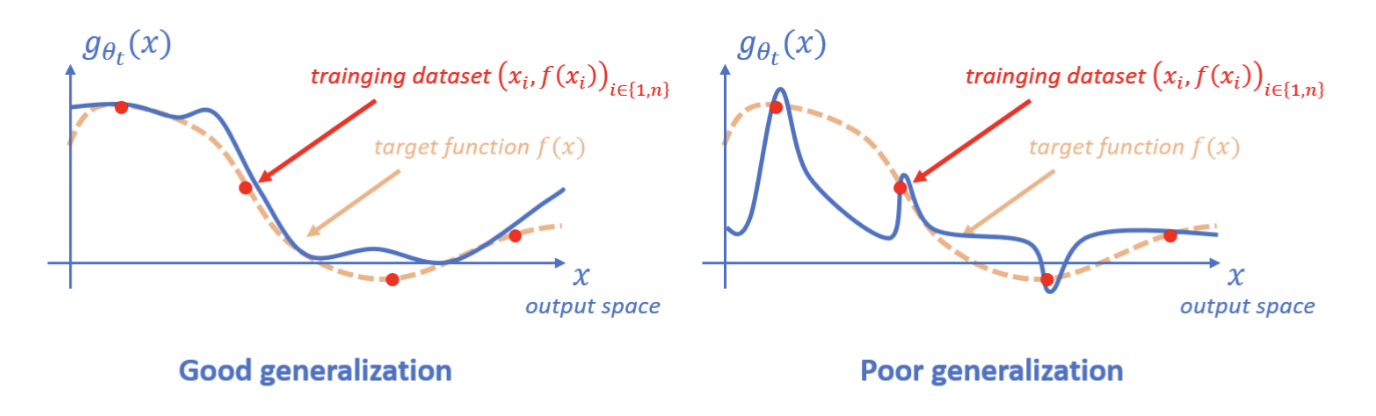
\includegraphics[width=\textwidth]{regularity-robustness/generalization.png}
    \caption{Generalization for different model regularity.}
    \label{fig:generalization}  
\end{figure}
A good intuition is that the more regular the model is, the better it will generalize. In \autoref{fig:generalization}, the left model is more regular, and while performing worst on the training set, it performs better on the whole space.

\subsubsection{Training objective and risk minimization}
Let $g_\theta:\X\to\Y$ be a model and $\D$ be a distribution of data points in $\X\times\Y$. Our true goal is to minimize the loss $\L_\D$:
\begin{equation*}
    \min_{\theta\in\R^d}\L_\D(\theta) = \E_{(X,Y)\sim\D}[\ell(g_\theta(X),Y)]
\end{equation*}
Nevertheless, during training we actually minimize $\L_{\hat{\D}_n}(\theta)$, where:
\begin{equation*}
    \hat{\D}_n := \frac{1}{n}\sum_{i=1}^n\delta(x_i, y_i)
\end{equation*}
is the empirical distribution over the training dataset $(x_i,i)_{i\in\iset{1}{n}}$.

Usually, the training set is not the final target: our objective is to provide a good model on another distributin $\D_{\textnormal{test}}$. This raises multiple sub-problems, depending on the test distribution: generalization, out-of-distribution samples, but also robustness, interpolation and aversarial attacks\dots

\subsubsection{Generalization}
We consider a setup in which the training samples are drawn i.i.d~according to the target distribution $\D=\D_{\textnormal{test}}$. Let:
\begin{equation*}
    \htheta_n = \argmin_\theta\L_{\hat{\D}}(\theta)
\end{equation*}
be the parameter minimizing the training loss. Assume that the model is sufficiently expressive, and therefore that $\L_{\hat{D}_n}(\htheta_n)=0$. The actual question is whether $\L_{\D}(\htheta_n)$ is small, i.e.~if the model generalizes well to the test distribution.

If $\theta\in\R^d$ is independent of the training samples, then, with probability $1-\delta$,
\begin{equation*}
    \left|\L_{\hat{\D}_n}(\theta)-\L_{\D}(\theta)\right| \leq \norm{\ell}_\infty \sqrt{\frac{2\ln(2/\delta)}{n}}
\end{equation*}
Unfortunately, $\htheta_n$ depends on the distribution $\hat{\D}_n$; therefore, we cannot apply the above majoration to $\theta=\htheta_n$.

\subsubsection{Decomposition of the error}


\subsection{Robustness and adversarial attacks}
\subsubsection{Adversarial attacks}
Consider a pre-trained model, achieving good results for a specific task, such as image classification. The idea of \emph{adversarial attacks} is to add small, invisible noise to an image to try to make the prediction of the model change.
\begin{figure}[H]
    \centering
    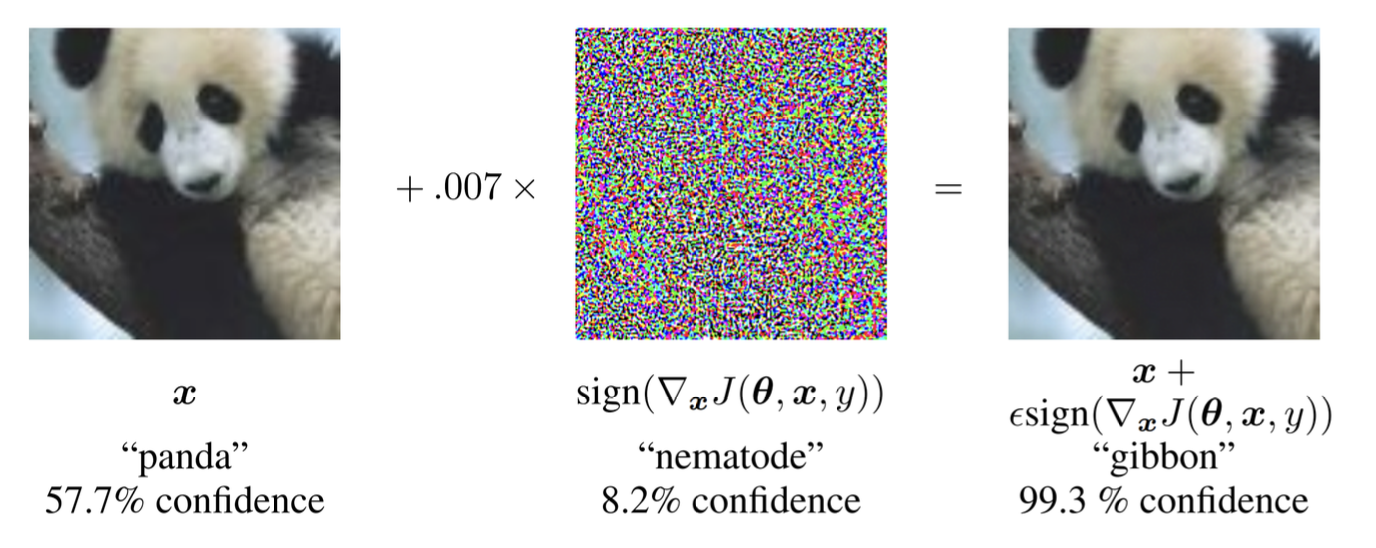
\includegraphics[width=.8\textwidth]{regularity-robustness/panda-attacks.png}
\end{figure}
In general, vision models are robust to random input noise: if an image of random noise is generated, the confidence score of the classification will be low. Nevertheless, most vision models are also extremely fragile to well-crafted input noise: that is, noise specifically designed (using for instance an optimization algorithm) to have a high confidence score for a specific class.

There are multiple types of adversarial attacks. White-box attacks use the knowledge of the model (such as its weights, for instance) to create the perturbation; it generally uses gradient descent on an objective different from the training objective: for instance, we might want to optimize the fact that this image is classified as a specific class. Black-box attacks do not have access to the parameters of the model; a frequently used technique is to create a white-box attack on a similar model, hoping that the optimization result will also work for the original model.

A model can be protected from attacks to some extent. A wide-spread approach is to augment the dataset with adversarial attacks; the model having seen a larger number of examples, some of which being attacked, it becomes more robust to later attacks. Another approach is to control the robustness, or smoothness, of the model. 

\subsubsection{Robustness of neural networks}
Protecting models from such attacks is vital for practical applications in engineering or medicine. If the model acts as a black-box, then trusting the model requires hard constraints. Intuitively, a robust model is such that a small input perturbation leads to a small output perturbation.

Formally, we can write a first order approximation of our model $g_\theta$:
\begin{equation*}
    g_\theta(x+\epsilon)-g_\theta(x) = J_{g,x}(x,\theta)\cdot\epsilon+o(\norm{\epsilon})
\end{equation*}
Control on the operator norm of the model,
\begin{equation*}
    \norm{J_{g_\theta}(x)} := \max_{u\neq0}\frac{\norm{J_{g_\theta}(x)u}_2}{\norm{u}_2}
\end{equation*}
leads to robustness. If we introduce the Lipschitz constant $L_{g_\theta}$ of the model:
\begin{equation*}
    L_{g_\theta} := \sup_x \norm{J_{g_\theta}(x)}
\end{equation*}
then maintaining a \say{small} Lipschitz constant guarantees small input perturbations to have limited output perturbations. For piece-wise linear interpolation, the Lipschitz constant is smaller than the target function. Nevertheless, for neural networks, we have:
\begin{equation*}
    L_{g_\theta} \leq\prod_lL_{f^{(l)}}
\end{equation*}
and can be exponential in the number of layers.

\newpage